
\begin{figure}[hpt!]
\centering
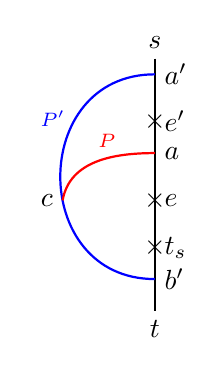
\begin{tikzpicture}[scale=2]

\definecolor{dgreen}{rgb}{0.0, 0.5, 0.0}
\begin{scope}[xshift=0cm]
\coordinate (s) at (0,1.6);
\coordinate (t) at (0,0);
\coordinate (ts) at (0,0.4);
\coordinate (b1) at (0,.2);

\coordinate (a1) at (0,1.5);
\coordinate (a) at (0,1);
\coordinate (v) at (0,0.7);
\coordinate (v1) at (0,1.2);
\coordinate (c) at (-0.585,0.7);

\draw[thick](s)--(t);
\node[above] at (s){$s$};
\node[below] at (t){$t$};
\node[right] at (a1){$a'$};
\node[right] at (a){$a$};
\node[right] at (b1){$b'$};
\node[left] at (c){$c$};


\draw[blue,thick] (a1) to[out=180,in=180,distance=.8cm] node[pos=0.3,left]
{\scriptsize  $P'$}  (b1);

\draw[red,thick] (a) to[out=180,in=80]
node[pos=0.4,above]
{\scriptsize  $P$}  (c);

\node at (v1){$\times$};
\node[right] at (v1){$e'$};

\node at (v){$\times$};
\node[right] at (v){$e$};

\node at (ts){$\times$};
\node[right] at (ts){$t_s$};
\end{scope}

\end{tikzpicture}

\caption{$\DET(P)$ intersects first with $\DET(P')$ at $c$ where  $P'
\in (>P)$.}
\label{fig:singlesecondcase}
\end{figure}
